% ****** Start of file template-TIF360-FYM360-blindtext.tex ******
%
% use on Overleaf!!!!
%
\documentclass[%
 reprint,
 amsmath,amssymb,
 aps,
]{revtex4-2}

\usepackage{subcaption} % Essential for subfigure environment


\usepackage{graphicx}% Include figure files
\usepackage{dcolumn}% Align table columns on decimal point
\usepackage{bm}% bold math
\usepackage{hyperref}% add hypertext capabilities
%\usepackage[mathlines]{lineno}% Enable numbering of text and display math
%\linenumbers\relax % Commence numbering lines
\usepackage{xcolor}

\usepackage{lipsum}

\begin{document}

\title{AI for Three-Body Problem Trajectory Prediction: \\
A Comparative Study of TCN, Reservoir and LSTM}
%%%A Comparative Study of Temporal Convolutional Networks, Reservoir and Long-Short-Term Memory Networks}

\author{Esben Almkvist}


\date{\today}% It is always \today, today,
             %  but any date may be explicitly specified

\begin{abstract} %%% DO NOT CHANGE!
%%% - B1 - %%%%%%%%%%%%%%%%%%%%%%%%%%%%%%%%%%% 
%%% Customize this part: text between - B1 - and - E1 - must not appear in the final report 
\noindent The three-body problem stands as a classic example of chaos theory, representing perhaps the simplest physical system that exhibits chaotic behavior. In this study, the three-body problem is simulated in two dimensions and machine learning models to predict its dynamics are developed. Multiple approaches are explored, including one-dimensional temporal convolutional networks , basic long-short-term memory networks, and reservoir models. The reservoir models trained rapidly and produced the best results for short forecasts, while the temporal convolutional networks performed best for longer forecasts. By combining temporal convolutional networks and reservoir models the overall best results were achieved. The Lyapunov time for the dimensionless three-body system was calculated to 2.49, highlighting the inherent limit of long-term predictability.


%%%%% Some notes:
\iffalse
\begin{itemize}
    \item Abstract: Classic three body problem. Create simulation data with physical model and train and forecast using three different neural network models. Predict trajectories. Three models. Classic RNN LSTM and Specialized TCN, and Reservoir. The latter two performed best. The TCN would predic the general trajectories accurate, but not the interaction of the bodies.
\end{itemize}
\fi

%%% - E1 - %%%%%%%%%%%%%%%%%%%%%%%%%%%%%%%%%%%%%%

\begin{description} %%% DO NOT CHANGE!
\item[Project Topic] %%% DO NOT CHANGE!
{Project K\\
Three Bodies, Three Models: Chaotic Time Series Analysis with Machine
Learning.} %CHANGE accordingly
\item[Teaching Assistant] %%% DO NOT CHANGE!
{Alex Lech} % CHANGE accordingly
\end{description} %%% DO NOT CHANGE!
\end{abstract}

\maketitle




\section{\label{sec:intro}Introduction} %%% DO NOT CHANGE!

%%% - B2 - %%%%%%%%%%%%%%%%%%%%%%%%%%%%%%%%%%% 
%%% Customize this part: text between - B2 - and - E2 - must not appear in the final report 
The three-body problem is a classic problem in physics, exhibiting chaotic behavior \cite{birkhoff1927dynamical}. In the early days of computing N-body systems ($N>2$) were used as an example to evaluate computational stability using different numerical formats, e.g. floats, double precision, etc \cite{DejongheAndHut1986}. One paper \cite{Breen_2020} claimed to have solved the three-body problem using an artificial neural network, probably a Multi-Layer Perceptron, but limited the results to bodies with initial speeds of 0. The work on the three-body problem was continued using a physics-informed neural networks (PINN) \cite{pereira2025advancingsolutionsthreebodyproblem}.
%was criticized for exaggerating the results \cite{LiLiLiao2020}. 
The prediction of chaotic systems, like weather and turbulent flows, remains a major challenge in both physics and machine learning due to their sensitivity to initial conditions. In several papers the chaotic Lorenz 63 or 96 systems are used for testing the performance of neural network models \cite{vlachas2018data, Chattopadhyay2019} and Kuramoto-Sivashinsky equation (used for flame propagation) in \cite{pathak2018model, vlachas2018data}. The three-body problem may not be as useful for neural network training due to its disruptive behavior when bodies collide or escape.

Time series forecasting have traditionally used recurring neural networks (RNNs) as best practice \cite{vlachas2018data}, but recently several other approaches have proved capable of matching the performance of the RNNs. In particular, reservoir computing (RC) has emerged as a compelling model-free strategy \cite{pathak2018model, Chattopadhyay2019}, offering the ability to learn temporal dynamics, even in chaotic systems. One-dimensional temporal convolutional networks (TCN) often outperform canonical RNNs such as long-short-term memory (LSTM) networks in multiple sequence modeling tasks \cite{bai2018empiricalevaluationgenericconvolutional, luo2024moderntcn}. 


The aim of this study is to evaluate the ability of three neural network architectures to forecast the trajectories of the bodies in the three-body system. Rather than trying to classify the system outcome, the focus is on learning an accurate time evolution of the dynamics of the system.

%%%%% Some notes:
\iffalse
\begin{itemize}
    \item Introduction: Three body problem is not refered to in previous studies of neural networks. Probably because of its chaotic behavior and disruptive behavior when bodies collide or escape. When two or all three objects are very close and the distance approaches zero, the gravitation becomes very large and an object is often catapulted out of the system; at least when simulated with a finite time step. A more common approach is using the Lorenz system to simulate a chaotic system that resembles natural phenomena, such as weather.
\end{itemize}
\fi

%% Get a better citation than Kobayashi

%%% - E2 - %%%%%%%%%%%%%%%%%%%%%%%%%%%%%%%%%%%%%%






\section{\label{sec:overview}Overview} %%% DO NOT CHANGE!

%%% - B3 - %%%%%%%%%%%%%%%%%%%%%%%%%%%%%%%%%%% 
%%% Customize this part: text between - B3 - and - E3 - must not appear in the final report 
Several data-driven models have been proposed for forecasting chaotic time series, each with trade-offs in complexity, interpretability, and performance. These are listed in table \ref{tab:methodsoverview}.

\begin{table*}
    \caption{\textbf{Overview of time-series forecasting methods for chaotic systems.} Summary of commonly used methods, their features, and suitability.}
    \label{tab:methodsoverview}
    \begin{tabular}{|p{2cm}|p{3cm}|p{6cm}|p{6cm}|}
    \hline
       \textbf{Method}  &  \textbf{Use case scenario}   &  \textbf{Features}  &  \textbf{Suitable for the project?}   \\
    \hline
        RC  & Chaotic time-series forecasting & Simple training; good short-term prediction; low interpretability; sensitive to hyperparameters \cite{pathak2018model, Chattopadhyay2019} & Yes. Best balance of performance and efficiency for model-free prediction.  \\
    \hline
        LSTM & High-dimensional spatiotemporal systems & Capable of long-term memory; data-hungry; harder to interpret \cite{vlachas2018data} & Moderate. Selected as a standard model used for timeseries forecasting.  \\
    \hline
        TCN & Chaotic and multiscale time series & Good for sequence modeling with long memory and parallel computation; interpretable; requires careful tuning \cite{bai2018empiricalevaluationgenericconvolutional} & Yes. Offers complementary strengths to RC and LSTM for medium- to long-term forecasting. \\
    \hline
        PINN & Nonlinear partial differential equations & A promising methodology is PINN \cite{RAISSI2019686}, which could be used as an alternative to forecasting the system. & No. Since the simulated system was not physically sound as the energy was not conserved. \\
    \hline
    \end{tabular}
\end{table*}

Given the trade-offs, three models were selected for implementation and comparison: RC, LSTM, and TCN. The PINN approach was excluded due to the lack of energy conservation in the simulated system. LSTM was chosen as a classical baseline for time series forecasting, given its strength in modeling recurrent patterns. TCN, a modern 1D convolutional neural network architecture, was included due to its recent success in outperforming traditional RNNs on multiple tasks. Finally, RC was selected for its demonstrated effectiveness in forecasting chaotic dynamics.

%%%%% Some notes:
\iffalse
\begin{itemize}
    \item Overview:   When simulating time series using neural networks a classical approach is to use RNNs as they are good at capturing recurring phenomena. Therefore a LSTM was used to represent the classical method for time series forecasting. In recent years 1D CCNs have been used to forecast time series with success, often performing better than traditional RNN methods. A modern TCN was used as the second model. Reservoir models have proven to be good at predicting the behavior of chaotic systems, so that was chosen as the third model.
\end{itemize}
\fi

%%% - E3 - %%%%%%%%%%%%%%%%%%%%%%%%%%%%%%%%%%%%%%




\section{\label{sec:method}Method} %%% DO NOT CHANGE!

%%% - B4 - %%%%%%%%%%%%%%%%%%%%%%%%%%%%%%%%%%% 
%%% Customize this part: text between - B4 - and - E4 - must not appear in the final report 

\subsection{Data Generation}

The three-body system was simulated in 2D with varying initial velocity in the x and y directions, with Newtonian gravity and numerically integrated motion using the Leapfrog method. The system was dimensionless with a gravitational constant of 1. Two of the bodies had similar masses, whereas the third had half the mass.
Each simulation was labeled as: 

\begin{itemize}
    \item \texttt{converging} - figure \ref{fig:classes} (a): A collision occurs when the distance between any two bodies is less than or equal to the sum of their radii.
    
    \item \texttt{diverging} - figure \ref{fig:classes} (b): A simplified form of Birkhoff's escape criterion \cite{birkhoff1927dynamical} was used. A system was considered diverging when the total energy of a body exceeded a threshold $\varepsilon$, set to 2:
    \[
    \underbrace{\frac{1}{2}m_i v_i^2}_{\text{Kinetic Energy}} \underbrace{-\sum_{i \ne j} \frac{G m_i m_j}{r_{ij}}}_{\text{Potential Energy}} > \varepsilon
    \] 
    where $m_i$ is the mass of body $i$, $v_i$ its speed, $G$ the gravitational constant, and $r_{ij}$ the distance between bodies $i$ and $j$.

    \item \texttt{stable} - figure \ref{fig:classes} (c): The system is considered stable if it completes 800 time-steps (each of size 0.01) without any collisions or escapes.
\end{itemize}


\begin{figure}
\centering
    \begin{minipage}{0.15723\textwidth}
        \centering
        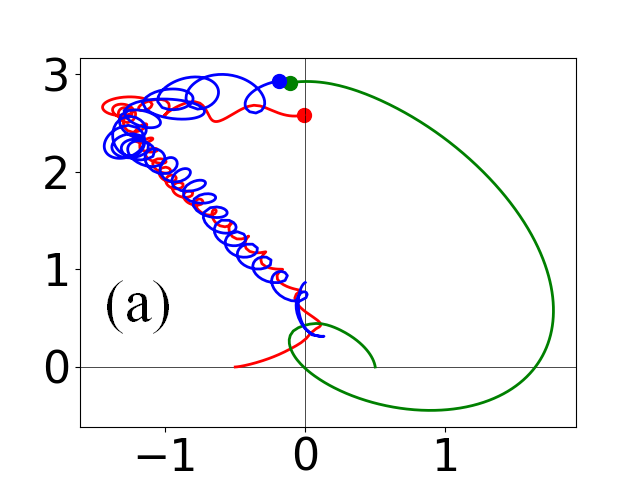
\includegraphics[width=\linewidth]{threebodies_15_marked.png}
    \end{minipage}
    \hfill
    \begin{minipage}{0.15723\textwidth}
        \centering
        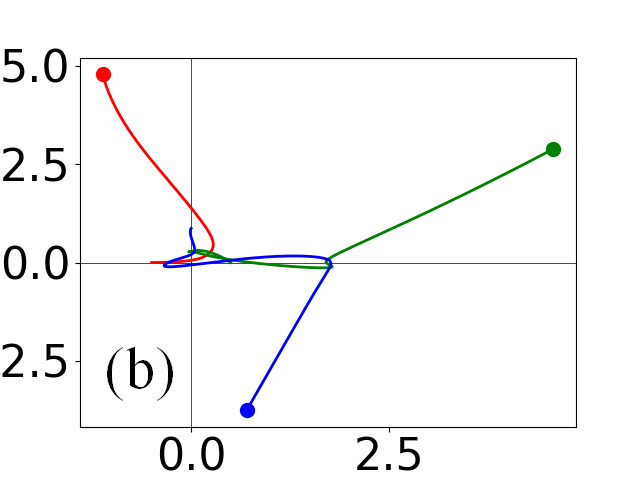
\includegraphics[width=\linewidth]{threebodies_14_marked.png}
    \end{minipage}
    \hfill
    \begin{minipage}{0.15723\textwidth}
        \centering
        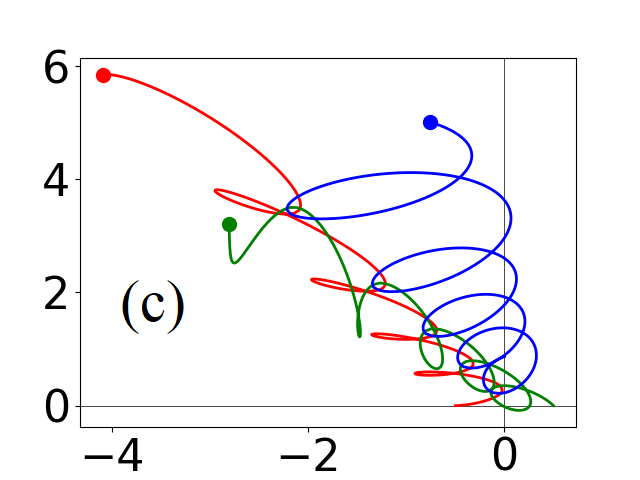
\includegraphics[width=\linewidth]{threebodies_13_marked.png}
    \end{minipage}

\caption{\textbf{Three body simulation.} The simulated trajectories for the three bodies for the different classes (a) converging, (b) diverging and (c) stable.}
\label{fig:classes}    
\end{figure}

The original goal of classifying system outcomes from predicted trajectories was revised due to uneven simulation lengths, limited model accuracy, and the inability to resolve fine differences between collisions and escapes. Therefore, only simulations reaching 800 time-steps were used in the training of the neural networks. That resulted in 2352 sequences which was divided into 1881 for training and 235 each for validation and testing. Time series of positions and velocities were extracted for all three bodies, giving input and output sequences of 200 and 600 time-steps respectively.


\subsection{Modeling Approaches}
Two approaches for time series forecasting were tested. The first was to predict the state of the system one time step ahead, then iteratively predict the next step based on previous predictions, until the final state of the system. The next approach was to predict the entire forecast horizon at once. The latter proved to be most successful, so all models were adapted to forecast the full future trajectory of the three-body system over 600 time-steps, with 12 variables per step (positions and velocities of three bodies in 2D). 

\begin{figure}
    \centering
    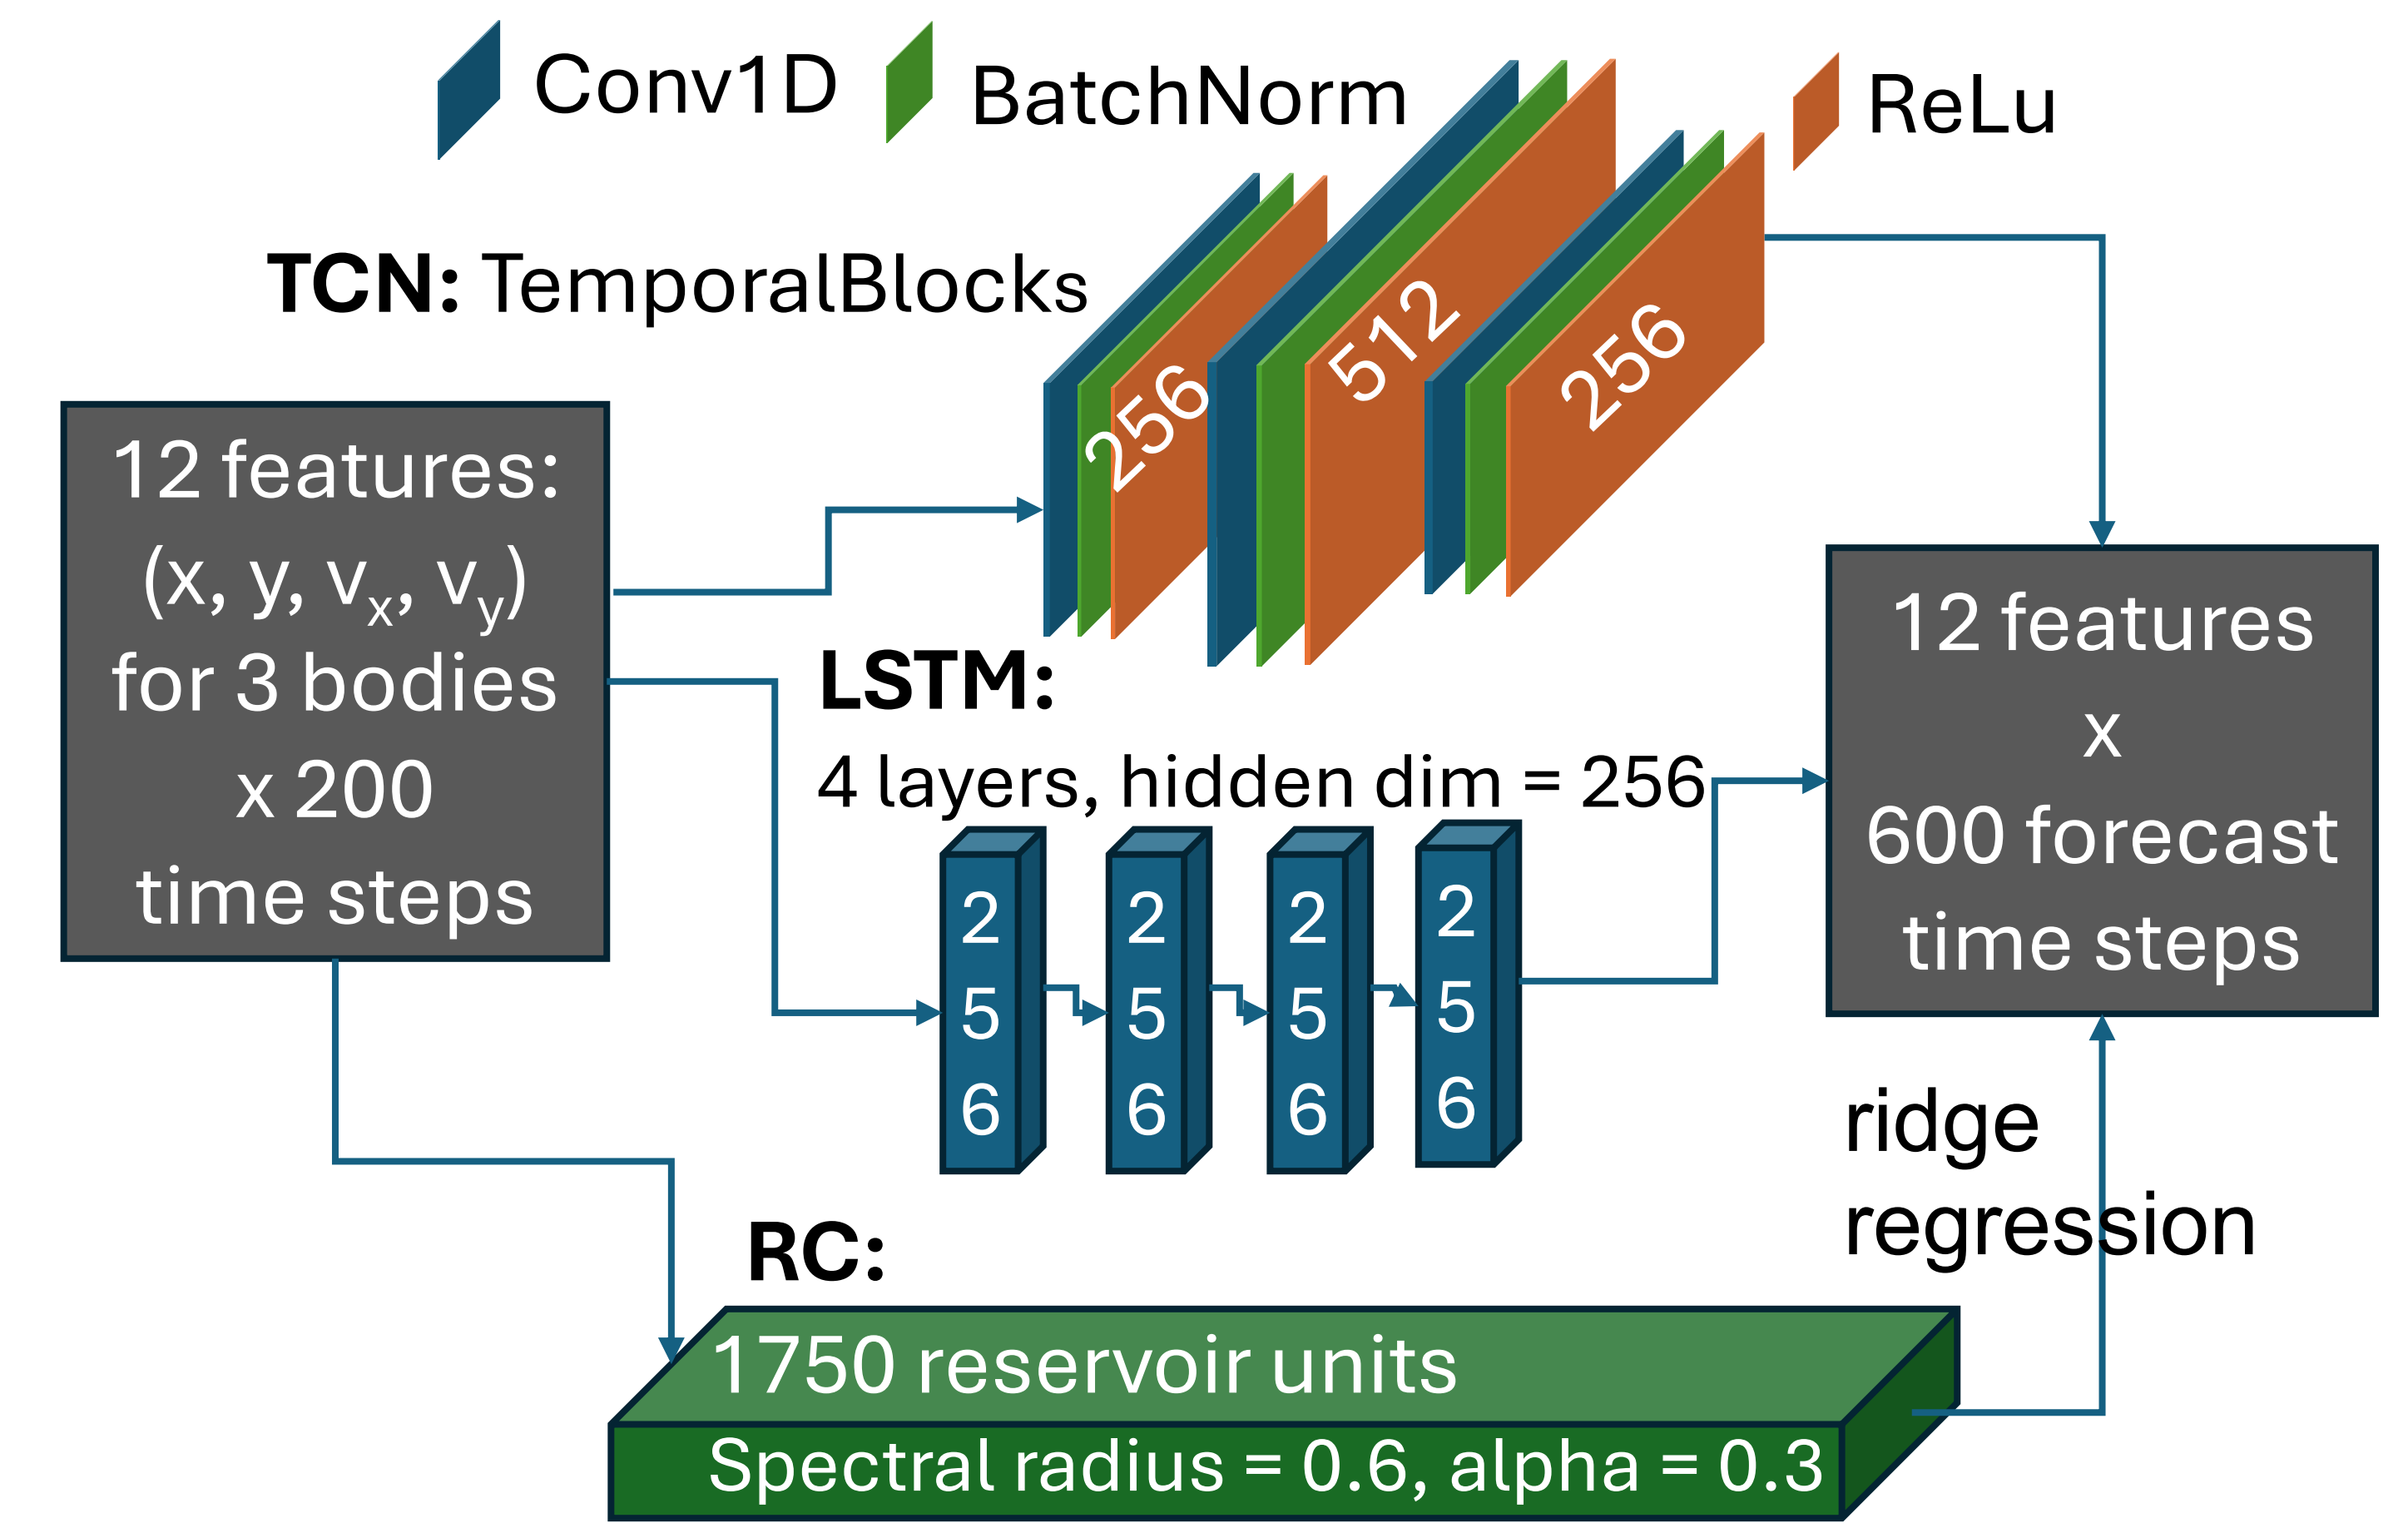
\includegraphics[width=0.99\linewidth]{MethodOverview.png}
    \caption{{\bf Overview of the three models.} The input sequence (gray box) was processed by three model types: TCN, LSTM, and RC. The TCN consisted of three TemporalBlocks with kernel size 3 and dilations of 1, 2, and 4. All models produced output in the same format (gray box): a 600-step forecast of 12 features.}
    \label{fig:methodoverview}
\end{figure}

%Models are shown in figure \ref{fig:methodoverview}.


A 4-layer LSTM with 256 hidden units was used to model temporal dependencies. The final hidden state initializes a decoder, which generates the full 600-step forecast. A fully connected layer maps each step to a 12-dimensional output; see figure~\ref{fig:methodoverview}.


The TCN uses three dilated 1D convolutional layers with hidden sizes [256, 512, 256], kernel size 3, and dilations 1, 2, and 4. Each layer includes batch normalization, ReLU activation, and residual connections. The final output is produced via a linear layer and reshaped to $(600, 12)$; see figure~\ref{fig:methodoverview}.


An Echo State Network with a fixed 1750-unit reservoir was used for model-free forecasting. The reservoir state is updated by applying a tanh activation to a weighted sum of the input and previous state, while the output is a linear projection of the reservoir. Only the output weights are trained, using ridge regression; see figure~\ref{fig:methodoverview}.


Finally, as it was realized that the TCN and RC models had different skills, they were joined to a combined model (TCN+RC), where the TCN would use its ability to predict the long-time state of the system and the RC would predict the residuals and thereby improve the forecast.

The Lyapunov time was calculated to relate the time to other chaotic systems and natural phenomena. This was done by perturbing one of the initial positions by $10^{-8}$ and looking at the distance between objects in the perturbed system compared to the original. A Model Time Unit (MTU) was calculated by fitting a line to a part of the system where the log of distance increased linearly. 

Furthermore, the energy should be conserved in the system, so to see how it behaved, the kinetic and potential energy were calculated for the simulation and for the neural network models.

\iffalse
\begin{itemize}
    \item Method: Describe data generation and selecting stable, converging and diverging systems. Show and describe the figures. 800 steps maximum. Input sequence length and forecasting 600 time-steps. Also tested a regressive method, only forecasting one timestep and forecasting the next step based on the forecasted data. This was abandoned as the forecasting in one go performed better. Describe each neural network method and the theory of each. Initially the idea was to predict the trajectories of the objects and then, based on the trajectories, check if the objects would collide, escape or remain stable. However, due to three reasons, the study focuses on predicting the trajectories of the objects rather than classifying the outcome: Simulation length. When objects collide or escape, the simulation was terminated giving it a length shorter than that of the stable case. For the system to learn properly, it was better to use longer sequences of data, which would favor the stable case. The models did not perform well enough for a meaningful classification based on the trajectories. When the bodies passed very close, the difference between a collision and escape due to the catapulting effect was well below the accuracy of the models. Only the stable sequences with 800 time-steps were chosen train the neural network models. The Lyapunov time was calculated to relate the time to other chaotic systems and natural phenomena. Figure shows the Lyapunov lambda and time. A Model Time Unit (MTU) was calculated. The energy should be conserved in the system, so to see how it behaved, it was calculated for the simulation and for the neural network models.
\end{itemize}
\fi

%%% - E4 - %%%%%%%%%%%%%%%%%%%%%%%%%%%%%%%%%%%%%%





\section{\label{sec:results}Results and Discussion} %%% DO NOT CHANGE!

%%% - B5 - %%%%%%%%%%%%%%%%%%%%%%%%%%%%%%%%%%% 
%%% Customize this part: text between - B5 - and - E5 - must not appear in the final report 
The training time varied between models when trained on 2xT4 GPUs. The RC trained in seconds in one go, while the LSTM needed more than 500 epochs and about 1 hour to achieve reasonable results. The TCN and TCN+RC trained faster/epoch than the LSTM and would get good results and stop-early after about 100-150 epochs -- about 10 minutes.

As shown in figure \ref{fig:lyapunov}, the fitted line gives a Lyapunov time for the simulations of 2.49. This is analogous to about 3.75 days in real atmosphere forecasting \cite{Chattopadhyay2019}, so our forecast horizon of 600 time-steps corresponds roughly to 10 days. An MTU was defined and used in the figures, where 0 was set at the start of the forecast after 200 time-steps. 


%%%%%% Some notes:
\iffalse
\begin{itemize}
    \item Results and Discussion: Describe what is in the figures. The LSTM did not learn much of the system's behavior. The TCN was good at predicting the long term movement of the trajectories. The reservoir was able to predict the behavior of the bodies quite well, but would go wrong more often than the TCN in the long run. By combining the TCN to predict the development of the system and reservoir to predict the residuals to mimic the behavior of the bodies, one could get higher accuracy. The table shows that the TCN and reservoir perform much better than the LSTM. The figures show that two regimes, one where all three bodies interact with each other and one where two bodies circulate around each other while the third body is in its own orbit. This last behavior was often well predicted as to the general direction of the bodies, but the interaction between the bodies was only captured by the reservoir model. The energy was not conserved properly in the simulation due to a too large time step.
    \item Another approach could be to train the model to predict the positional change in each time step instead of the position itself. The distance to the other objects could also be used to make sure that the model will understand that something occurs when two bodies are close. As the simulation was stopped when two bodies collided or when the escape energy was large enough to escape, which occurred just after a close encounter of two or all three bodies, the model would never learn that the bodies are catapulted away during such occasions.
\end{itemize}
\fi

\begin{figure}
    \centering
            \begin{minipage}{0.2333\textwidth}
                \centering
                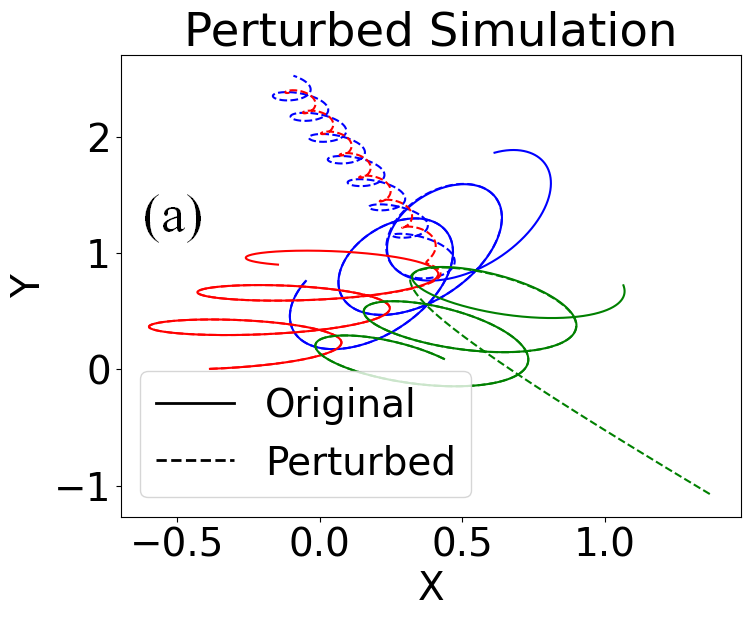
\includegraphics[width=\columnwidth]{Lyapunov_x_y_simulation_marked.png}
            \end{minipage}
            \hfill
            \begin{minipage}{0.2427\textwidth}
                \centering
                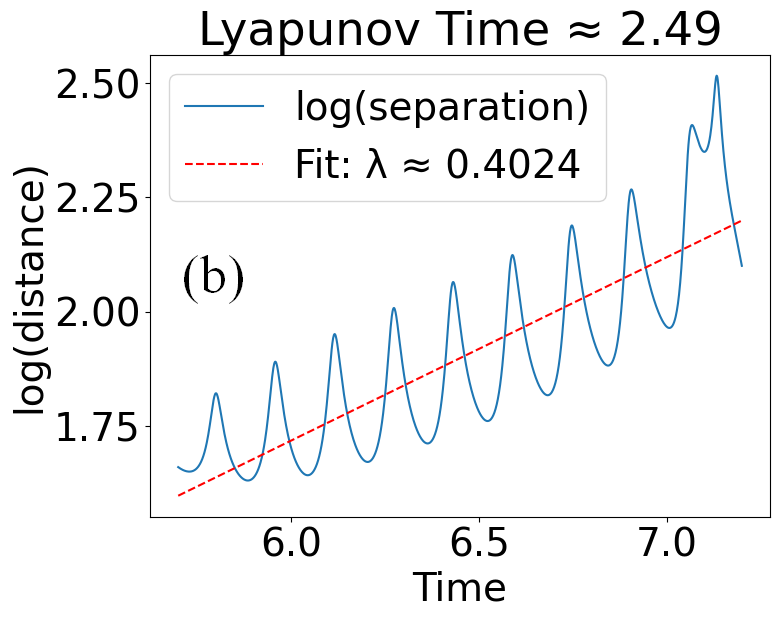
\includegraphics[width=\columnwidth]{Lyapunov_time_marked.png}
            \end{minipage}
    
    \caption{\textbf{Lyapunov time calculation.} The Lyapunov time was calculated for a period when the log of the separation was linear.(a) Position perturbed by $10^{-8}$ in the simulation. (b) Linear fitting to log of separation.}
    \label{fig:lyapunov}
\end{figure}

\begin{figure*}[htbp] % [htbp] is a common placement preference (here, top, bottom, page)
    \centering
    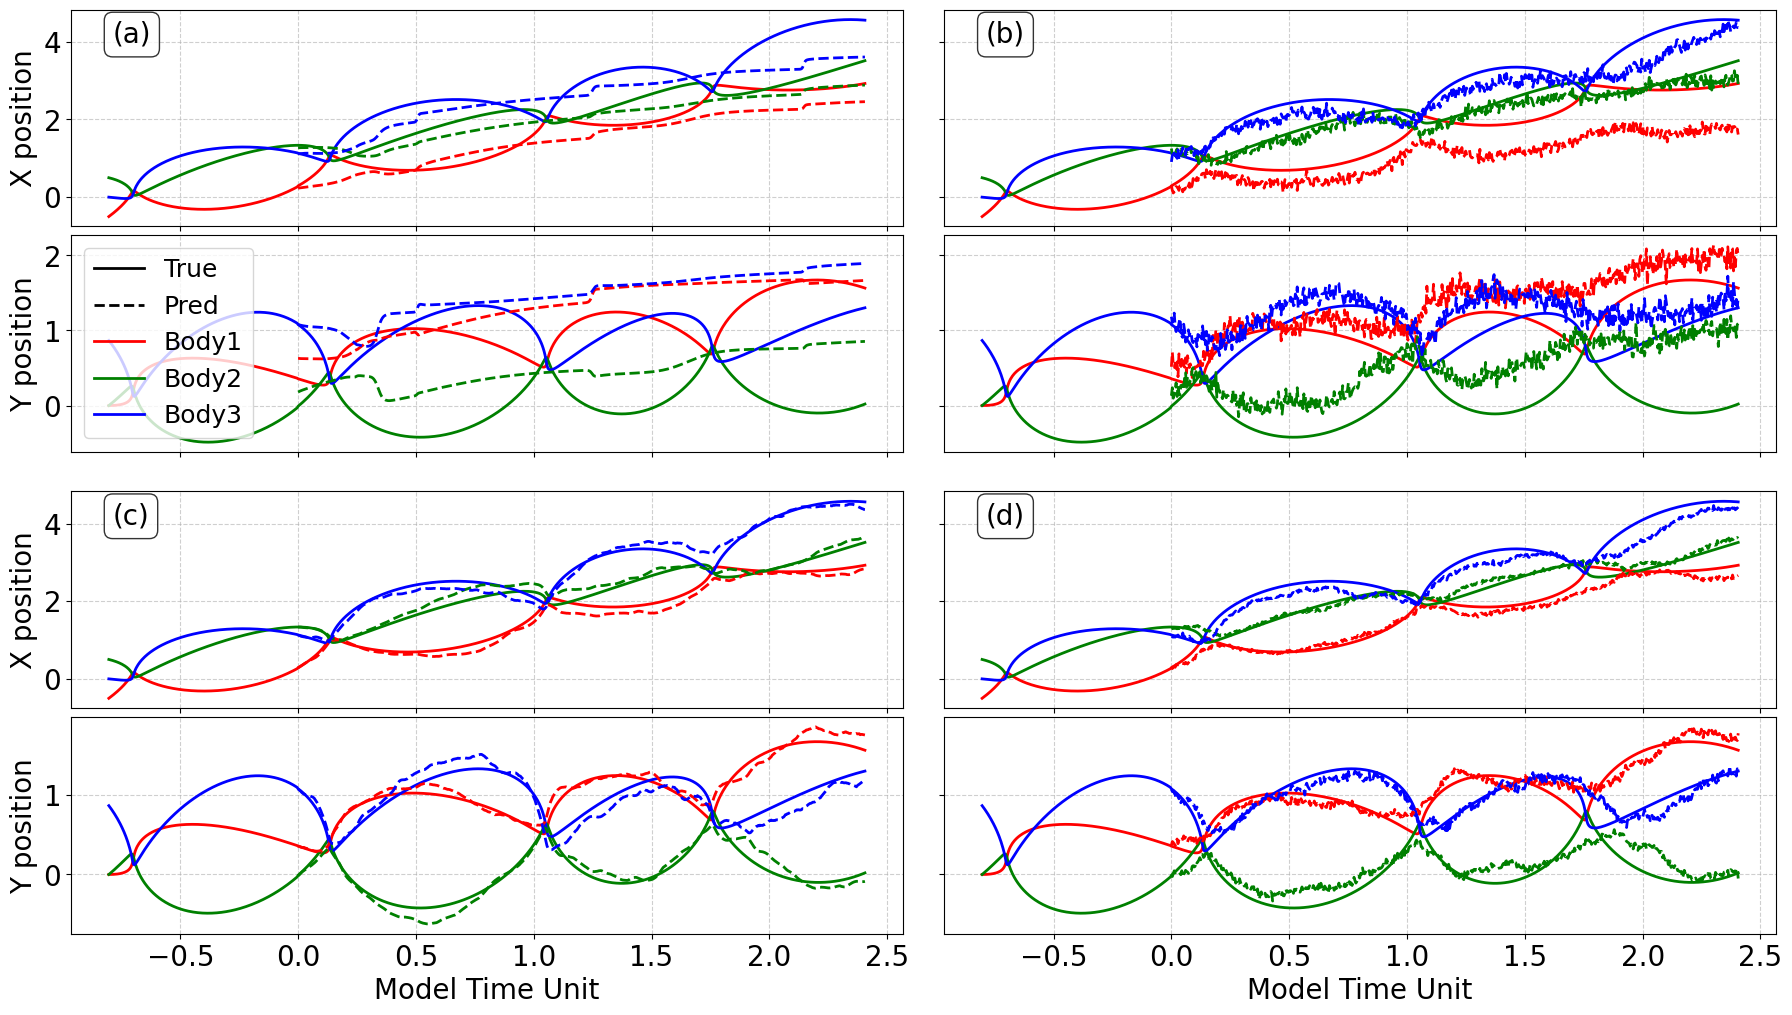
\includegraphics[width=\linewidth]{plot_1_Final_Allplots_22x12.png}
    \caption{\textbf{Performance of the models.} In this simulation all three bodies interacted. (a) LSTM, (b) TCN, (c) RC, and (d) TCN+RC.}
    \label{fig:prediction_set_1_results}
\end{figure*}


\begin{figure*}[htbp]
    \centering
    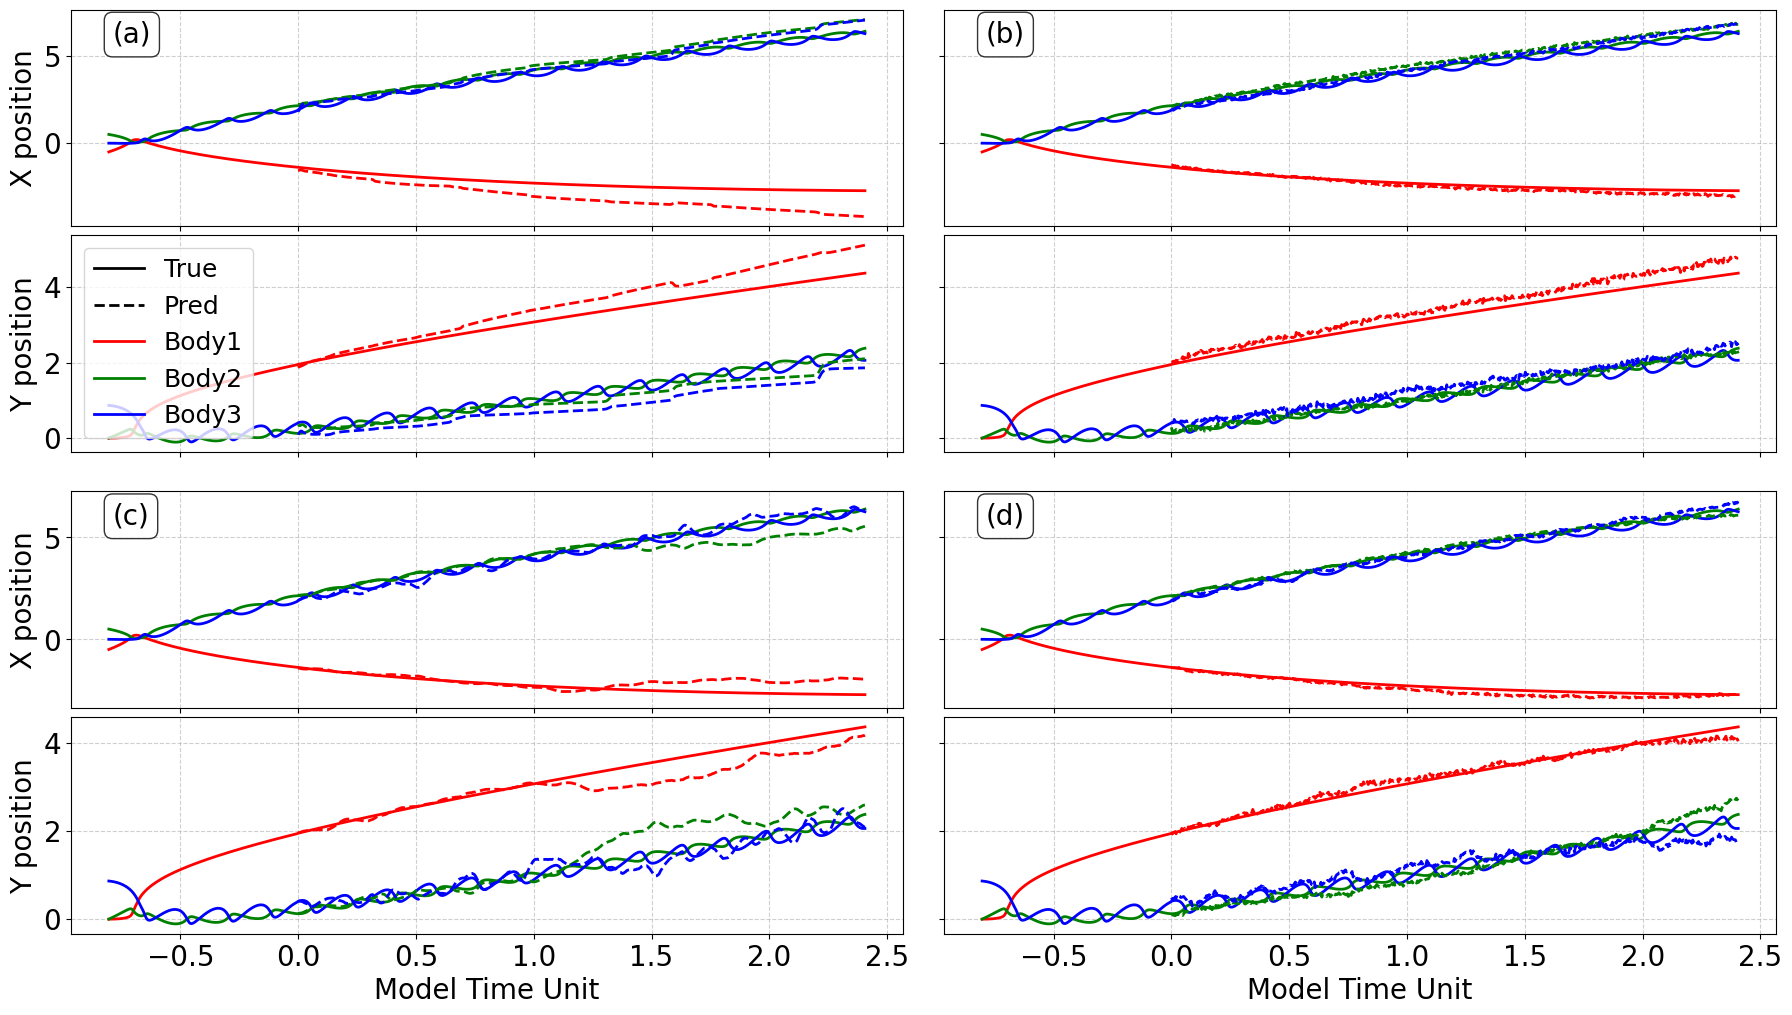
\includegraphics[width=\linewidth]{plot_3_Final_Allplots_22x12.png}
    \caption{\textbf{Performance of the models.} In this simulation one body was on its own path while the other two interacted. (a) LSTM, (b) TCN, (c) RC, and (d) TCN+RC.}
    \label{fig:prediction_set_2_results}
\end{figure*}



\begin{figure*}
    \centering
    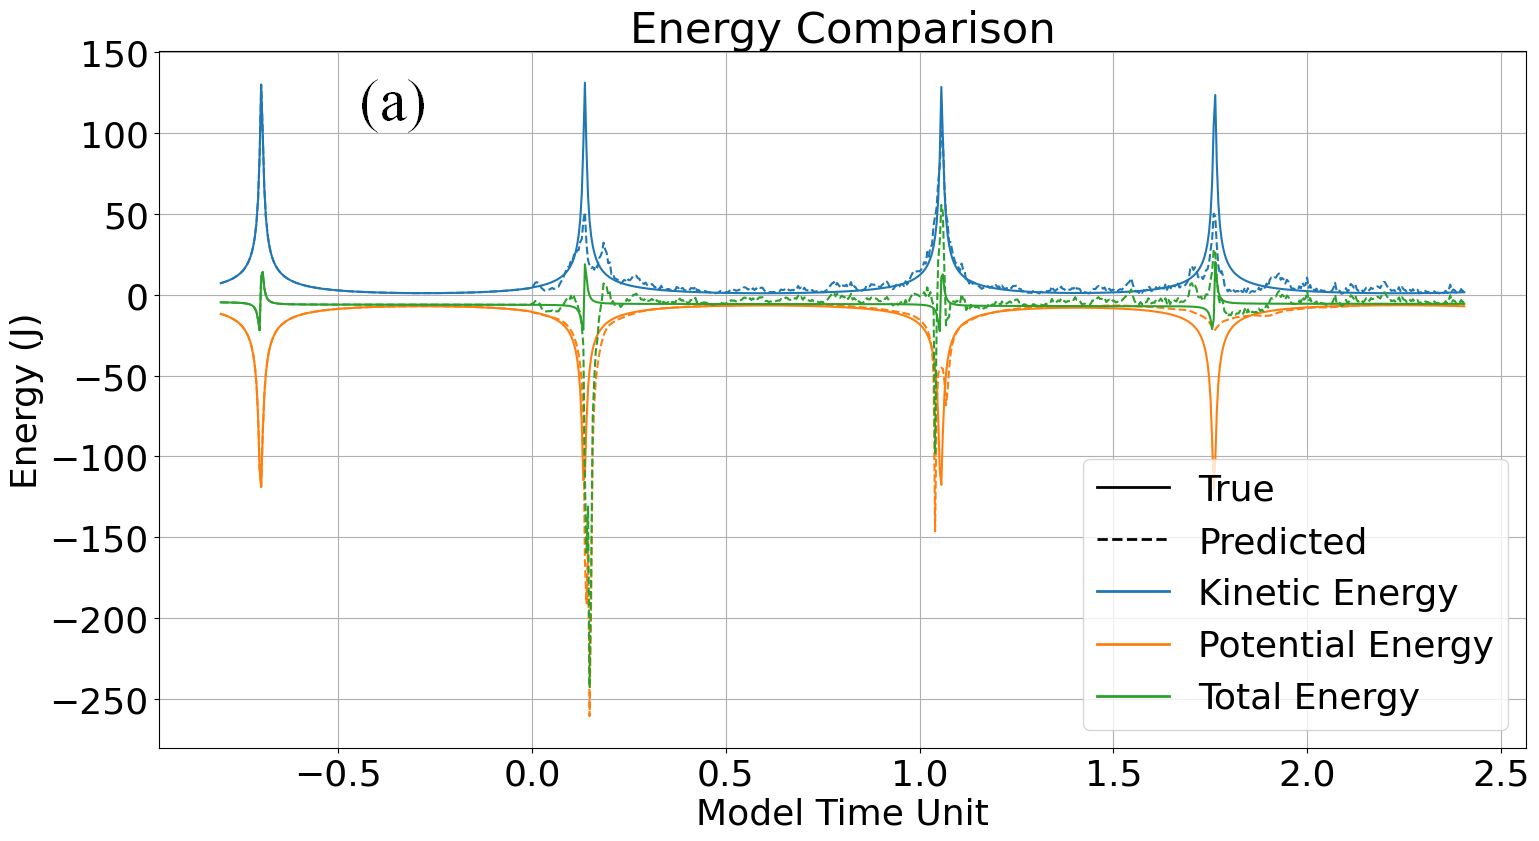
\includegraphics[width=0.497\linewidth]{plot_1_Energy_Reservoir_marked.png}
    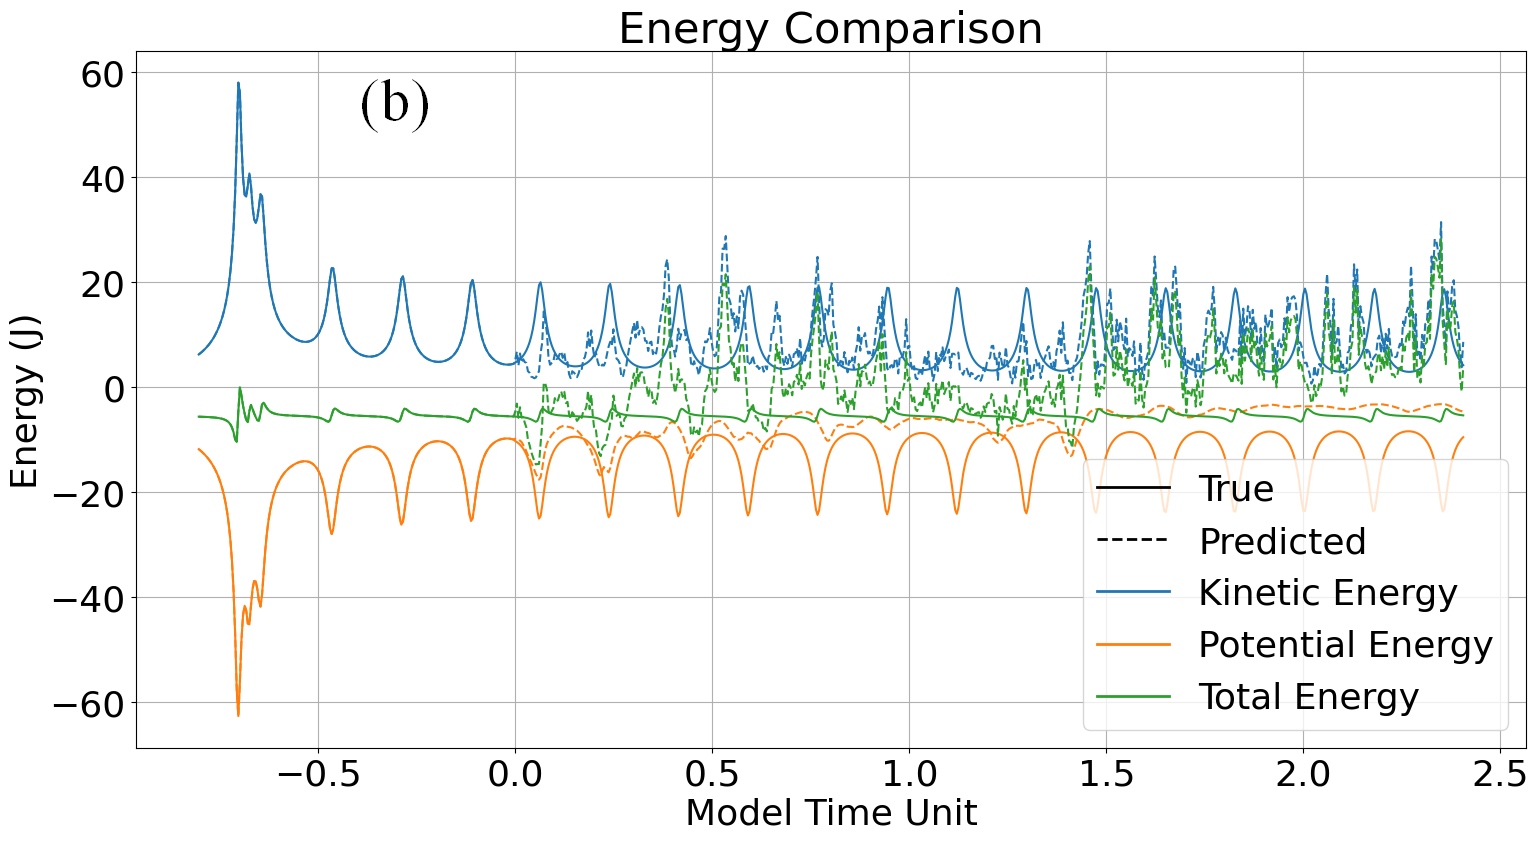
\includegraphics[width=0.497\linewidth]{plot_3_Energy_Reservoir_marked.png}
    \caption{\textbf{Energy Conservation:} The kinetic, potential, and total energy of all bodies are shown in the figure for both the simulation and the RC model. In the simulation, energy is not conserved when the bodies pass close to one another. The RC model does not conserve energy, but it does not drift. (a) and (b) show the same time series as figure \ref{fig:prediction_set_1_results} and \ref{fig:prediction_set_2_results} respectively.}
    \label{fig:energy}
\end{figure*}

The bodies typically had two types of behaviors; when all three bodies interacted as in figure \ref{fig:prediction_set_1_results} and when one body would go off in its own orbit, while the other two interacted with higher frequency, as in figure \ref{fig:prediction_set_2_results}. The second type was more common, so the LSTM model would focus on learning that type of behavior where it was enough to learn the general direction of the bodies to get a low loss. The TCN would learn the behavior of the bodies to some extent, but it was only the RC model that actually learned how the bodies interacted. This is consistent with previous observations \cite{pathak2018model}. The TCN has a very jagged curve compared to the others, probably due to the lack of temporal continuity, but the noise dampened in the TCN+RC model.

Table \ref{tab:distance_rmse_updated} shows the forecast quality for different forecast horizons. The RC performed best for short forecasts, but surprisingly, the TCN model, despite showing a higher error in the short term, eventually outperformed the RC at the longest forecast horizons (above 200 time-steps), indicating its potential for long-range temporal dependencies. By combining the TCN for the long-range forecast accuracy and an RC for predicting the interaction between the bodies, the best results were achieved. It is interesting that between 200 and 600 time-steps, the rmse increases to more than double, and as the Lyapunov time is 2.49 (249 time-steps), chaotic behavior should be more common beyond this point.

The energy of the system plotted in figure \ref{fig:energy} shows how the kinetic and potential energy interact when the bodies pass close to each other. Ideally, the energy should always be conserved, but in the simulated system, it is evident that during close encounters of two or more bodies, the energy departs from its normal state. Since the time step in the simulation is fixed, this is expected. For the neural network in the example, the energy varies a lot more than the simulated. If a PINN would be used to account for energy fluctuations, the results may improve, but one would need to make sure that the simulated data would conserve energy better, e.g. by decreasing the time step when the bodies are close to one another. %\cite{Szebehely1973}.


%%%% This is the table in use:
\begin{table}[htbp]
    \centering
    \caption{{\bf Distance RMSE results.} RC had the highest accuracy for short forecast horizons (H), but for longer forecasts TCN and TCN+RC performed better. LSTM was worse at all horizons.}
    \label{tab:distance_rmse_updated}
    \begin{tabular}{|l|c|c|c|c|c|c|}
        \hline
        \textbf{Model} & \textbf{H=1} & \textbf{H=25} & \textbf{H=50} & \textbf{H=100} & \textbf{H=200} & \textbf{H=600} \\
        \hline
        LSTM & 0.552 & 0.525 & 0.548 & 0.594 & 0.704 & 1.161 \\
        \hline
        TCN & 0.241 & 0.257 & 0.268 & 0.299 & 0.392 & 0.823 \\
        \hline
        RC & 0.035 & 0.152 & 0.204 & 0.277 & 0.436 & 1.024 \\
        \hline
        TCN+RC & 0.067 & 0.141 & 0.177 & 0.223 & 0.311 & 0.715 \\
        \hline
    \end{tabular}
\end{table}


%% Commenting this out with iffalse:
\iffalse
\begin{table}
    \caption{{\bf Overview of results for different forecast horizons.} Root Mean Square Error (RMSE) for position forecasts of three models at different horizons. 
} 
    \begin{tabular}{|c|ccc|ccc|ccc|}
        \hline
        \textbf{Forecast} & \multicolumn{3}{c|}{\textbf{Reservoir}} & \multicolumn{3}{c|}{\textbf{LSTM}} & \multicolumn{3}{c|}{\textbf{TCN}} \\
        \textbf{Horizon} & \multicolumn{3}{c|}{\textbf{Model}} & \multicolumn{3}{c|}{\textbf{Model}} & \multicolumn{3}{c|}{\textbf{Model}} \\
        \textbf{(time-steps)} & \textbf{x} && \textbf{y} & \textbf{x} && \textbf{y} & \textbf{x} && \textbf{y} \\
        \hline
        1   & 0.095 && 0.075 & 0.376 && 0.388 & 0.406 && 0.425 \\
        25  & 0.148 && 0.158 & 0.406 && 0.399 & 0.426 && 0.433 \\
        50  & 0.196 && 0.198 & 0.440 && 0.411 & 0.441 && 0.443 \\
        100 & 0.251 && 0.259 & 0.499 && 0.446 & 0.470 && 0.472 \\
        200 & 0.355 && 0.379 & 0.627 && 0.552 & 0.541 && 0.546 \\
        \hline
    \end{tabular}
    \label{tab:rmse_forecast}
\end{table}
\fi

\iffalse
\begin{table}[htbp]
    \centering
    \caption{Distance RMSE Results for Different Models and Forecast Horizons}
    \label{tab:distance_rmse}
    \begin{tabular}{|l|c|c|c|c|c|c|}
        \hline
        \textbf{Model} & \textbf{H=1} & \textbf{H=25} & \textbf{H=50} & \textbf{H=100} & \textbf{H=200} & \textbf{H=600} \\
        \hline
        LSTM & 0.865 & 0.637 & 0.616 & 0.613 & 0.683 & 1.270 \\
        \hline
        TCN & 0.355 & 0.341 & 0.355 & 0.377 & 0.466 & 0.885 \\
        \hline
        Reservoir & 0.037 & 0.158 & 0.204 & 0.265 & 0.398 & 1.002 \\
        \hline
        Combined & 0.068 & 0.144 & 0.184 & 0.232 & 0.321 & 0.728 \\
        \hline
    \end{tabular}
\end{table}
\fi

\iffalse
\begin{table}[h]
    \centering
    \caption{RMSE of Predicted Positions $(x, y)$ for Each Model Across Forecast Horizons}
    \begin{tabular}{|c|cc|cc|cc|}
        \hline
        \textbf{Horizon} & \multicolumn{2}{c|}{\textbf{Reservoir Model}} & \multicolumn{2}{c|}{\textbf{LSTM Model}} & \multicolumn{2}{c|}{\textbf{TCN Model}} \\
        \cline{2-7}
         & $x$ & $y$ & $x$ & $y$ & $x$ & $y$ \\
        \hline
        1   & 0.024 & 0.026 & 0.513 & 0.424 & 0.159 & 0.162 \\
        25  & 0.093 & 0.116 & 0.424 & 0.365 & 0.172 & 0.179 \\
        50  & 0.124 & 0.150 & 0.442 & 0.384 & 0.185 & 0.193 \\
        100 & 0.177 & 0.181 & 0.497 & 0.416 & 0.222 & 0.206 \\
        200 & 0.276 & 0.303 & 0.623 & 0.489 & 0.274 & 0.248 \\
        600 & 0.687 & 0.740 & 1.316 & 0.882 & 0.488 & 0.563 \\
        \hline
    \end{tabular}
    \label{tab:rmse_results}
\end{table}
\fi

%%% - E5 - %%%%%%%%%%%%%%%%%%%%%%%%%%%%%%%%%%%%%%




\section{\label{sec:conclusion}Conclusions and Outlook} %%% DO NOT CHANGE!

%%% - B6 - %%%%%%%%%%%%%%%%%%%%%%%%%%%%%%%%%%% 
%%% Customize this part: text between - B6 - and - E6 - must not appear in the final report 

Due to the complexity of the chaotic system with three moving objects and their interactions, machine learning models had trouble classifying the outcome of the system. LSTMs struggled to learn anything apart from the general direction of the bodies. Although model-free approaches such as RC were most reliable and showed promise in predicting the trajectories of the bodies, convolutional architectures like TCNs show promising long-term forecasting capabilities, especially when combined with the skills of the RC model. Future work could look at training the model to predict the positional change in each time step instead of the position itself. In addition, by explicitly including the distance to other objects in the training, the model would better understand the interaction between two or more bodies. Another approach could be to investigate more hybrid architectures, incorporate PINNs as in \cite{RAISSI2019686}, or enforce energy constraints explicitly during training to further improve generalization and physical correctness. 

\iffalse
\begin{itemize}
    \item Conclusions and Outlook: TCN and RC outperformed the LSTM. The RC was able to capture the behavior of the system while the TCN was good at capturing the general direction of the bodies. By combining those two, the system performed quite well.
    By using a smaller time step, one could make sure that the energy was conserved in the system. Physical laws could be introduced in the loss function to make sure that the trained model would behave according to physical laws. 
\end{itemize}
\fi

%%% - E6 - %%%%%%%%%%%%%%%%%%%%%%%%%%%%%%%%%%%%%%
\iffalse
\begin{table}
    \begin{center}
        \caption{\bf This is just kept as a reminder and making sure I don't exceed 5 pages.}
        \begin{tabular}{|c|c|c|c|c|c|}
        \hline
            \raisebox{0pt}[13pt][6pt]{\hspace*{3pt}} \parbox[c][][c]{1.2cm}{\textbf{Project team}} & 
            \raisebox{0pt}[13pt][6pt]{\hspace*{3pt}} \parbox[c][][c]{1.0cm}{\textbf{Pages}} & 
            \raisebox{0pt}[13pt][6pt]{\hspace*{3pt}} \parbox[c][][c]{1.2cm}{\textbf{Refs (min)}} & 
            \raisebox{0pt}[13pt][6pt]{\hspace*{3pt}} \parbox[c][][c]{1.2cm}{\textbf{Refs (max)}} & 
            \raisebox{0pt}[13pt][6pt]{\hspace*{3pt}} \parbox[c][][c]{1.2cm}{\textbf{Figs (min)}} & 
            \raisebox{0pt}[13pt][6pt]{\hspace*{3pt}} \parbox[c][][c]{1.2cm}{\textbf{Figs (max)}} 
        \\
        \hline
            \raisebox{0pt}[13pt][6pt]{\hspace*{3pt}} 1 &   5 & 5 & 10 & 3 & 6  \\   
        \hline
            \raisebox{0pt}[13pt][6pt]{\hspace*{3pt}} 2 &   9 & 10 & 20 & 5 & 9  \\   
        \hline
            \raisebox{0pt}[13pt][6pt]{\hspace*{3pt}} 3 &  13 & 15 & 30 & 7 & 11 \\       
            \hline
        \end{tabular}
    \end{center}
\end{table}
\fi


\section{\label{sec:Contribution}Contributions} %%% DO NOT CHANGE!

%%% - B7 - %%%%%%%%%%%%%%%%%%%%%%%%%%%%%%%%%%% 
%%% Customize this part: text between - B7 - and - E7 - must not appear in the final report 
The author solely implemented the code, performed the data analysis and wrote the manuscript.

%%% - E7 - %%%%%%%%%%%%%%%%%%%%%%%%%%%%%%%%%%%%%%

\section{\label{sec:COI}Conflict of Interest} %%% DO NOT CHANGE!

%%% - B8 - %%%%%%%%%%%%%%%%%%%%%%%%%%%%%%%%%%% 
%%% Customize this part: text between - B8 - and - E8 - must not appear in the final report 
The author declares no conflict of interest.

%%% - E8 - %%%%%%%%%%%%%%%%%%%%%%%%%%%%%%%%%%%%%%

\section{\label{sec:datacode}Data and Code Availability} %%% DO NOT CHANGE!

%%% - B9 - %%%%%%%%%%%%%%%%%%%%%%%%%%%%%%%%%%% 
%%% Customize this part: text between - B9 - and - E9 - must not appear in the final report 
All code and datasets used in this project are available at: \href{https://github.com/ebsbel/threebody}{https://github.com/ebsbel/threebody}.

%%% - E9 - %%%%%%%%%%%%%%%%%%%%%%%%%%%%%%%%%%%%%%
%%% - B10 - %%%%%%%%%%%%%%%%%%%%%%%%%%%%%%%%%%% 
%%% Customize this part: text between - B10 - and - E10 - must not appear in the final report 
%%% - E10 - %%%%%%%%%%%%%%%%%%%%%%%%%%%%%%%%%%%%%%


\bibliography{biblio-TIF360-FYM360} %%% DO NOT CHANGE!
% Produces the bibliography via BibTeX.

\end{document}
